% !TEX TS-program = pdflatexmk
\documentclass{styles/assisi}
\DeclareRobustCommand{\DelivNumber}{Camera calibration}
\DeclareRobustCommand{\DelivName}{\today}
\DeclareRobustCommand{\DelivStatus}{Confidential}
\DeclareRobustCommand{\DelivRevision}{0.1}
\DeclareRobustCommand{\DeliveryDate}{}
\DeclareRobustCommand{\DelivPartnersOwning}{\bf EPFL}
\DeclareRobustCommand{\DelivPartnersContributing}{\bf PARIS7}
\DeclareRobustCommand{\DelivPartnersContributingNextLine}{}
\DeclareRobustCommand{\DelivDue}{N/A}
\DeclareRobustCommand{\DelivAbstract}{This tutorial explains how to calibrate a new camera in CATS2.}

%----------------------------------------------------------------------------------------------
\makeindex

\usepackage{epsfig,subfigure,float,pseudocode,multirow,footmisc,rotating}
\usepackage{graphicx}        % standard LaTeX graphics tool
\usepackage{amsmath, amssymb, subfigure}
\usepackage{multirow, rotating}
\usepackage[ruled,lined,commentsnumbered]{algorithm2e}
\usepackage[colorlinks=false, urlcolor=blue, pdfborder={0 0 0}]{hyperref}
%\usepackage{algorithm2e}
\usepackage{pdfpages}
\usepackage{afterpage}
\usepackage{booktabs}
\usepackage{geometry}
\usepackage{listings}
\usepackage{color}

\newcommand{\rd}{\Delta^{\frac{1}{2}}}
\newcommand{\pla}{\phi_{\lambda_1}^t}
\newcommand{\plb}{\phi_{\lambda_2}^t}
\newcommand{\ie}{i.\,e.,\ }
\newcommand{\Ie}{I.\,e.,\ }
\newcommand{\eg}{e.\,g.,\ }
\newcommand{\Eg}{E.\,g.,\ }
\newcommand{\assisi}{ASSISI$|_{bf}$ }
\setcounter{tocdepth}{3}

% TODO command
\newcommand{\todo}[1]{\par\noindent{\raggedright\textsc{\color{red}#1}%
    \par\marginpar{{\Large\color{red}$\star$}}}}

\begin{document}
\thispagestyle{plain}
  \vspace*{0.3cm}
  \begin{center}
  {\bf \LARGE SEVENTH FRAMEWORK PROGRAMME}\\
  \vspace*{0.6cm}
  
\includegraphics[width=0.15\textwidth]{styles/7th.png}\\
  \vspace*{2.0cm}
  \bf {\large IP}\\
  \vspace*{1.0cm}
  \bf {\Huge ASSISIbf}\\
  \vspace*{.6cm}
  \bf {\it \Large Animal‌ and‌ robot‌ Societies‌ ‌Self-organise‌ and‌ Integrate‌ by‌ Social‌ Interaction‌ (bees‌ and‌ fish)‌}\\
  \vspace*{45pt}
  {\huge \bf \DelivNumber}\\
  \vspace*{12pt}
  {\Large \it \bf \DelivName}\\
  \vspace*{70pt}
  \small
  \begin{tabular}{|ll|}
    \hline &\\
    Date of preparation: \DeliveryDate & Revision: \DelivRevision\\ &\\
    Start date of project: February 1st, 2013 & Duration: 60 months\\ &\\
    Project co-ordinator: UNIGRAZ & Classification: \DelivStatus \\ &\\
    Partners: & \\
    %& \\
    ~~{\it owning:} \DelivPartnersOwning &~~{\it contributed:} \DelivPartnersContributing\\
    &\DelivPartnersContributingNextLine\\
    &\\
    Project website: & http://assisi-project.eu\\
    &\\
    \hline
  \end{tabular}
  \end{center}
%\newpage
%
%%-----------------------------------------------------------------
%\begin{center}
%\begin{tabular}{|lp{10cm}|}
%\hline &\\
%\multicolumn{2}{|c|}{\bf \Large DELIVERABLE SUMMARY SHEET} \\
%&\\
%\hline \hline
%&\\
%Project Number: & 601074\\
%&\\
%Project Acronym: & {\bf ASSISIbf}\\
%&\\
%Title:     & Animal‌ and‌ robot‌ Societies‌ ‌Self-organise‌ and‌ Integrate‌ by‌ Social‌ Interaction‌ (bees‌ and‌ fish) \\
%&\\
%\hline \hline
%&\\
%Deliverable N$^o$: & \DelivNumber\\
%&\\
%Due Date: & Project month: \DelivDue\\
%&\\
%Delivery Date: & \DeliveryDate \\
%&\\
%\hline \hline
%&\\
%\textbf{Name:} & {\bf \DelivName}\\
%&\\
%\textbf{Description:} & \DelivAbstract\\
%&\\
%&\\
%\hline \hline
%&\\
%Partners owning: & \DelivPartnersOwning \\
%&\\
%&\\
%Partners contributed: & \DelivPartnersContributing ~\DelivPartnersContributingNextLine \\
%&\\
%&\\
%Made available to: & \DelivStatus\\
%&\\
%\hline
%\end{tabular}
%\end{center}
%%}{}



%------------------------------------------------------------------



\textsf{\tableofcontents}
%\textsf{\listoffigures}
%\addcontentsline{toc}{chapter}{List of Figures}
%\textsf{\listoftables} \addcontentsline{toc}{chapter}{List
%of Tables}

\lstset{
    language=xml,
    tabsize=3,
    %frame=lines,
    %caption=Test,
    %label=code:sample,
    %frame=shadowbox,
    %rulesepcolor=\color{gray},
    xleftmargin=20pt,
    framexleftmargin=15pt,
    %keywordstyle=\color{blue}\bf,
    %commentstyle=\color{OliveGreen},
    %stringstyle=\color{red},
    numbers=left,
    numberstyle=\tiny,
    numbersep=5pt,
    breaklines=true,
    showstringspaces=false,
    basicstyle=\footnotesize}

\chapter{Introduction}\label{chap:intro}
In this tutorial we will show how to calibrate new camera for CATS2. The calibration consists of two parts: setting up the intrinsic and extrinsic parameters. 

The calibration files are stored in the {\it config/camera-calibration} folder. As an example have a look on the {\it epfl-setup-180} folder.

\chapter{Finding good parameters}\label{chap:calibration}
\section{Setting intrinsic parameters}
Use the chessboard pattern that can be downloaded here \url{http://docs.opencv.org/2.4/doc/tutorials/calib3d/camera_calibration/camera_calibration.html}. 

You can use the code proposed on the above-mentioned OpenCV documentation webpage, or its Python version (like one here \url{http://opencv-python-tutroals.readthedocs.io/en/latest/py_tutorials/py_calib3d/py_calibration/py_calibration.html}). We recommend to use the camera calibration application that can be found here: \url{https://github.com/gribovskiy/opencv-camera-calibration}. This application exports the camera parameters in the {\it xml} format. 

In any case once you have the {\it camera matrix} and {\it distortion coefficients} you can put them to the camera calibration file, e.g. like in {\it cats2-epfl-180-angle-below-camera.xml}. Make sure that the camera frame size specified in the calibration {\it xml} file is the one that you used for the calibration and the one you will be using in the experiments.

\section{Setting extrinsic parameters}
Here we presume that you are calibration the camera for the fish-setup made at EPFL, and that you have the dedicated calibration frame (Fig. \ref{fig:calibration-frame}). First of all measure the distance from your camera sensor to the setup and put it into the {\it cameraHeight} value in the calibration file. Make sure that the units are specified correctly in the {\it worldUnits} value, CATS2 supports {\it mm}, {\it cm} and {\it m}. 

\begin{figure}[h]
\centering
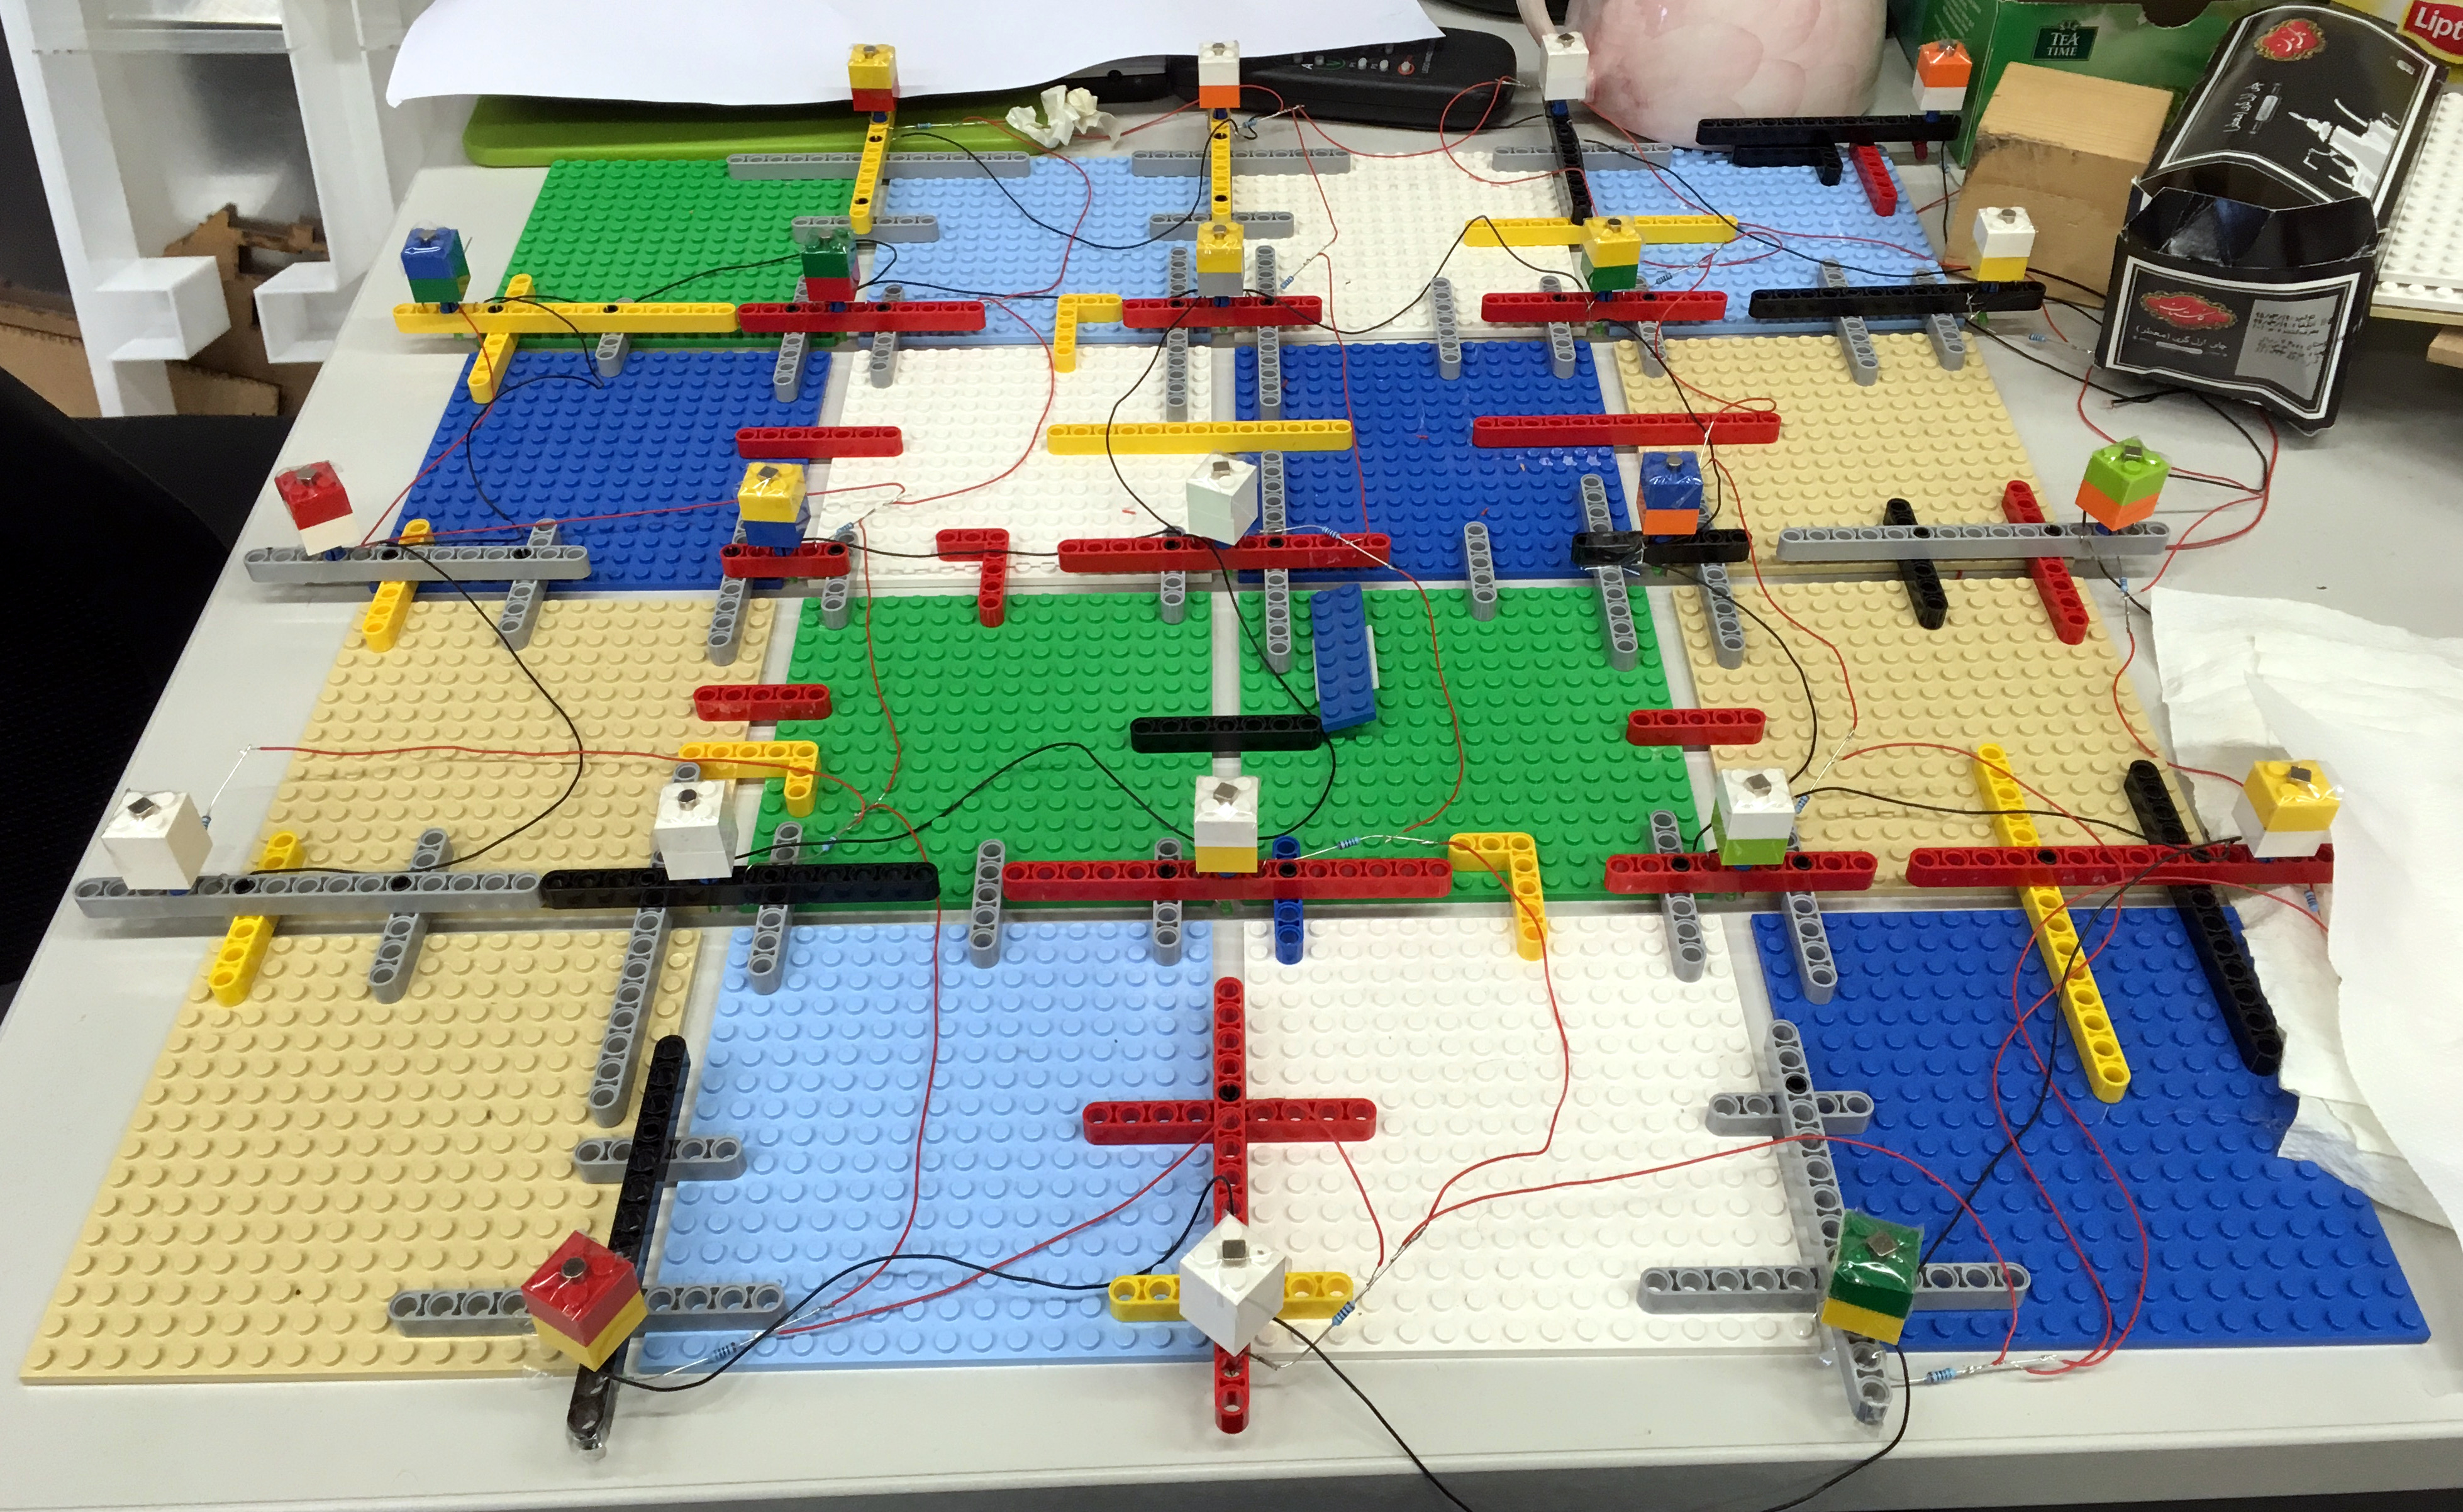
\includegraphics[width=0.65\textwidth]{./figs/calibration-frame}
\caption{The calibration frame. On top it has magnets placed on a grid, on the bottom every magnet has a corresponding LED.}
\label{fig:calibration-frame}
\end{figure}

Place the calibration frame under the aquarium and place the magnets into the aquarium in the locations corresponding to the magnets on the frame; the water level should be on the same level as for experiments. Take a print-screen (Fig. \ref{fig:main-setup}). 

\begin{figure}[h]
\centering
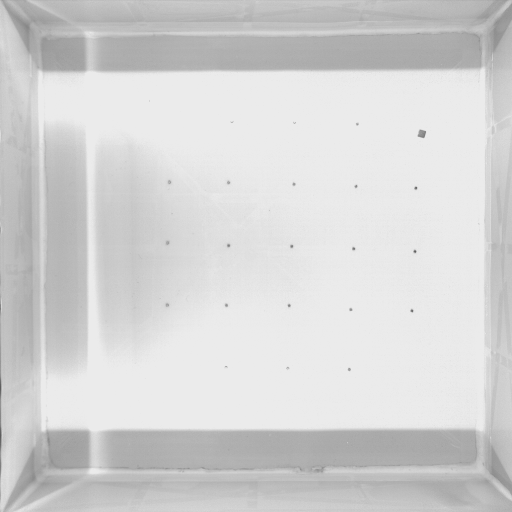
\includegraphics[width=0.65\textwidth]{./figs/cats2-main-camera}
\caption{The view of the main setup with the calibration pattern. The top-right magnet is used when we use two cameras, one above and another under the aquarium to synchronize them.}
\label{fig:main-setup}
\end{figure}

Take one of the vertices of the grid as the $(0,0)$ position. Here we assume that the $x$ axis goes to the right and the $y$ axis goes to the left. Note that if you calibrate two cameras simultaneously then the origin position should be the same for both. In this case the inversion parameters in the calibration {\it xml} files should be set as on the listing \ref{lst:inversion-flags}.

\begin{lstlisting}[caption={Axes invertion flags},label={lst:inversion-flags},language=xml]
<invertX>0</invertX>
<invertY>1</invertY>
\end{lstlisting}

Run the {\it pixel-locator} application from the CATS2 examples, load your print-screen and pick the pixel positions for every magnet, they are to be put to the calibration file along with the corresponding world positions. For an example, see {\it cats2-epfl-main-camera-basler.xml} file in the {\it config/camera-calibration/epfl-setup-180} folder. 

\section{Verifying the calibration}
The calibration file has to be specified in the {\it cameraCalibrationFile} value of the corresponding setup in the CATS2 configuration file, for an example see {\it cats2-epfl-setup.xml} file, and the section {\it setups/mainCamera/cameraCalibrationFile}. 

Then run {\it camera-viewer} example from CATS2 with the parameters 
{\it -mc if ../../../config/camera-calibration/epfl-setup-180/cats2-main-camera.png -bc if ../../../config/camera-calibration/epfl-setup-180/cats2-180-angle-below-camera.png  -c ../../../config/cats2-epfl-setup.xml -st mainCamera}. Here replace paths by your own calibration images for the main and the bottom (if used) setups and your configuration file. It will show the static main camera view on the screen. If you want to see the view from the bottom camera, then use {\it -st cameraBelow}. 

By pointing the cursor on the magnets check that the world coordinates are correct and thus the camera was correctly calibration. Also check the console output of {\it camera-viewer}, it should contain lines like {\bf "Average projection error (world->image) is 0.144409 pixels" (void CameraCalibration::calibrate(QString, QSize))} and {\bf "Average reprojection error (image->world) is 1.40595 mm" (void CameraCalibration::calibrate(QString, QSize))}, the error values should be reasonably low. 

\end{document}

